% Kompiuterijos katedros šablonas
% Template of Department of Computer Science II
% Versija 1.0 2015 m. kovas [ March, 2015]

\documentclass[a4paper,12pt,fleqn]{article}
\usepackage[unicode,colorlinks=false]{hyperref}


\usepackage[utf8x]{inputenc}
%

\usepackage[L7x]{fontenc}
\usepackage{times}
\usepackage{ucs}

 %package to switch the language
\usepackage{etoolbox}

  %set up of the page margins
\usepackage[top=2cm, bottom=2cm, left=3cm, right=1.5cm]{geometry}

 %1.1 line spacing
\linespread{1.1}


  %page numbering at the right side
\usepackage{fancyhdr}
\pagestyle{fancyplain}
\fancyhf{}
\renewcommand{\headrulewidth}{0pt} 
\fancyhfoffset[RO]{0cm}

  %to number at the bottom (exchange lines to number at the top)
\rfoot{\thepage}
  %\rhead{\thepage} %

% \usepackage[usenames,dvipsnames]{pstricks}
\urlstyle{same}
\hypersetup{
%  citecolor=Blue,
%  linkcolor=Blue,
%  urlcolor=Blue
pdfborder={0 0 0 }
}

 %for includegraphics
\usepackage{graphicx}



\usepackage[toc,page]{appendix}


\usepackage{caption}

 %for source codes
\usepackage{listings}
\lstset{commentstyle=\color{red},xleftmargin=10pt, framexleftmargin=6pt, numbersep=1mm, frame=single, numbers=left,numberstyle=\footnotesize,extendedchars=\true, inputencoding=utf8x,basicstyle=\footnotesize,extendedchars=true,
 keywordstyle=\color{black}\bfseries, breaklines=true, breakautoindent=true,framesep=8pt,linewidth=0.95\textwidth
}

 %for algorithms
\usepackage{algorithm}
\usepackage{algorithmic}
 %instead of the above two packages we can use algorithms2e
%\usepackage[boxed,linesnumbered,vlined,slide]{algorithm2e}

 %special symbols
\usepackage{amsfonts}
\usepackage{amssymb}
\usepackage{amsmath}

 %for theorem like environments
\usepackage{amsthm}

 \usepackage{datetime}
 \renewcommand{\dateseparator}{--}


% SI system units
\usepackage{siunitx}
\sisetup{detect-all}
% Problem with fonts \SI{x.xx}{\micro\metre}, solved with updmap-sys --enable Map=utm.map
\renewcommand{\sfdefault}{uhv}
\renewcommand{\rmdefault}{utm}
\renewcommand{\ttdefault}{ucr}

% List management (itemize, etc.)
\usepackage{enumitem}

\newcommand*{\urlw}[1]{\href{#1}%
            {\nolinkurl{#1}}}

\numberwithin{equation}{section}


\newtoggle{inLithuanian}
 %If the report is in Lithuanian, it is set to true; otherwise, change to false
\settoggle{inLithuanian}{false}

%create file preface.tex for the preface text
%if preface is needed set to true
\newtoggle{needPreface}
\settoggle{needPreface}{false}

\newtoggle{signaturesOnTitlePage}
\settoggle{signaturesOnTitlePage}{false}


\theoremstyle{definition}
\newtheorem{definition}{\keyWordDefinition}
\newtheorem{example}{\keyWordExample}
\def\QED{\unskip\nobreak\hfill\kern5pt$\Box$}

\iftoggle{inLithuanian}{
%\usepackage[L7x]{fontenc}
\usepackage[english,lithuanian]{babel}

\newcommand{\todayiso}{\the\year \dateseparator \twodigit\month \dateseparator \twodigit\day}


\renewcommand{\today}{\number\year\space m. \space \ifcase\month\or
  sausio\or vasario\or kovo\or balandžio\or gegužės\or birželio\or
  liepos\or rugpjūčio\or rugsėjo\or spalio\or lapkričio\or
  gruodžio\fi
  \space\number\day\space d.}


 \usepackage{tocloft}
 \renewcommand\cftsecaftersnum{.} 
 \renewcommand\cftsubsecaftersnum{.} 
 \renewcommand\cftsubsubsecaftersnum{.}

 \usepackage{VUMIFKK}

 \DeclareCaptionLabelFormat{captionlt}{#2 #1}
   %smth is not fine with algorithms 
 \DeclareCaptionLabelFormat{captionltalg}{#2 #1 algoritmas}

 \usepackage{indentfirst}
 \renewcommand{\appendixtocname}{Priedai}
 \renewcommand{\appendixpagename}{Priedai}
 \renewcommand{\contentsname}{Turinys} 

 \renewcommand{\lstlistingname}{išeities kodas}
 \renewcommand{\figurename}{pav}
 \renewcommand{\tablename}{lentelė}


 \captionsetup*[lstlisting]{   
 labelsep=period,labelformat=captionlt
 }
 \captionsetup*[figure]{   
% labelsep=period,
 labelsep=space, %babel redefines pav to pav.
 labelformat=captionlt
 }
 \captionsetup*[table]{   
  labelsep=period,
  labelformat=captionlt
 }
 \renewcommand{\algorithmicrequire}{\textbf{Įvestis:}}
 \renewcommand{\algorithmicensure}{\textbf{Išvestis:}}

 \captionsetup*[algorithm]{   
 labelsep=period,labelformat=captionltalg
 }

\renewcommand{\thmhead}[3]{#2 #1#3}

}
{
%\usepackage[OT1,T1]{fontenc}
%\usepackage[L7x]{fontenc}



\usepackage[english]{babel}
\newcommand{\todayiso}{\twodigit\month \dateseparator \twodigit\day \dateseparator \the\year}
 \captionsetup*[algorithm]{   
 labelsep=period
 }
\captionsetup*[lstlisting]{   
 labelsep=period
 }
 \captionsetup*[figure]{   
 labelsep=period
 }
 \captionsetup*[table]{   
 labelsep=period
 }


}

%some kywords
 \def\keywordAbstract{\iftoggle{inLithuanian}{Santrauka}{Abstract}}
 \def\keyWordIntroduction{\iftoggle{inLithuanian}{Įvadas}{Introduction}}
 \def\keyWordConclusions{\iftoggle{inLithuanian}{Išvados ir rekomendacijos}{Conclusions and Recommendations}}

 \def\keyWordPreface{\iftoggle{inLithuanian}{Pratarmė}{Preface}}
 \def\keyWordAppendice{\iftoggle{inLithuanian}{Priedas}{Appendix}}
 \def\keyWordSignature{\iftoggle{inLithuanian}{parašas}{signature}}
 \def\keyWordDefinition{\iftoggle{inLithuanian}{apibrėžimas}{Definition}}
 \def\keyWordExample{\iftoggle{inLithuanian}{pavyzdys}{Example}}


 %non-numbered sections: #1 param: for labeling sec:#1, #2 -section title
\newcommand{\sectionWithoutNumber}[2]{\newpage
%\hspace{2cm}
\section*{#1}
\label{sec:#2}
\addcontentsline{toc}{section}{\nameref{sec:#2}}%{#3}
 }



\newcommand{\referenceSources}[1]{
\newpage
\cleardoublepage
\phantomsection
\iftoggle{inLithuanian}{
 \renewcommand{\refname}{Literatūros šaltiniai}

 \addcontentsline{toc}{section}{Literatūros šaltiniai}
 \markboth{\refname}{Literatūros šaltiniai}
 }
{

\addcontentsline{toc}{section}{References}
\markboth{References}{References}
}

\bibliographystyle{plain}
\bibliography{#1}
}



 \newcommand\authorsignature[1]{
\begin{flushright}
 \begin{minipage}[b]{0.45\textwidth}
  \centering
  \rule{\textwidth}{0.5pt}\\
   #1
  \end{minipage}
\end{flushright}
 }




 \newcommand\authorsignatures[5]{%
   \vspace{1cm}
   \authorsignature{#1}
   \ifstrequal{#2}{}{}{\vspace{0.3cm}
     \authorsignature{#2}
     \ifstrequal{#3}{}{}{\vspace{0.3cm}
      \authorsignature{#3}
      \ifstrequal{#4}{}{}{\vspace{0.3cm}
        \authorsignature{#4}
        \ifstrequal{#5}{}{}{\vspace{0.3cm}
         \authorsignature{#5}       
        }
      }
    }
} 
}

\newcommand{\authortitle}{
\iftoggle{signaturesOnTitlePage}{
\tiny{\keyWordSignature}
}{}
}

\newcommand{\depttitlepage}[8]
{
\thispagestyle{empty}
\begin{center}


\includegraphics[width=2cm]{jb_VU_zenklas}

%\vspace{-1cm}

\iftoggle{inLithuanian}
{ 
  VILNIAUS UNIVERSITETAS\\
  MATEMATIKOS IR INFORMATIKOS FAKULTETAS\\
  INFORMATIKOS INSTITUTAS\\
  KOMPIUTERINIO IR DUOMENŲ MODELIAVIMO KATEDRA
}
{
  VILNIUS UNIVERSITY \\
  FACULTY OF MATHEMATICS AND INFORMATICS \\
  INSTITUTE OF COMPUTER SCIENCE\\
  DEPARTMENT OF COMPUTATIONAL AND DATA MODELING
}

\vspace{5cm}

#1\\
\vspace{0.5cm}
\textbf{\Large #2}
\end{center}

\vspace{5cm}


\hspace{0.5\textwidth}
\begin{minipage}{0.4\textwidth}
 \begin{flushleft} 
\iftoggle{inLithuanian}
{
 \ifstrequal{#3}{}{}{Atliko:\\[5pt]}
}
{
\ifstrequal{#3}{}{}{Done by:\\[5pt]}
}

%\noindent
\begin{tabular}{@{}lr}%\setlength\tabcolsep{0pt}
\ifstrequal{#3}{}{}{#3&\hspace{2cm}\authortitle\\[5pt]}
\ifstrequal{#4}{}{}{#4&\authortitle\\[5pt]}
\ifstrequal{#5}{}{}{#5&\authortitle\\[5pt]}
\ifstrequal{#6}{}{}{#6&\authortitle\\[5pt]}
\ifstrequal{#7}{}{}{#7&\authortitle\\[5pt]}
\ifstrequal{#8}{}{}{#8&\authortitle\\}
\end{tabular}

\end{flushleft}

\end{minipage}

\vspace{0.5cm}
\hspace{0.5\textwidth}
\begin{minipage}{0.4\textwidth}
 \begin{flushleft} 


\end{flushleft}

\end{minipage}


\vfill

\begin{center}
Vilnius\\
\the\year
\end{center}

\iftoggle{needPreface}{
 \sectionWithoutNumber{\keyWordPreface}{preface}
Pratarmės (Preface) informacija


\iftoggle{inLithuanian}
{
\vspace{\baselineskip}\hfill
\today
}
{
 \vspace{\baselineskip}\hfill \today
}

 \vspace{5cm}

\iftoggle{signaturesOnTitlePage}{}
{
\authorsignatures{#3}{#4}{#5}{#6}{#7}
}
}{}
\newpage
}


\begin{document}
 % #1 -report type, #2 - title, #3-7 students,
 \depttitlepage{Software engineering project}{Degantisvaskas}{Domantas Nėjus, - Leader}{Mindaugas Zinkevičius,}{Eimantas Rimkus,}{Lukas Drobelis,}{Audrius Miškinis,}{Arijus Uleckas}% students 2-5

\tableofcontents


 %the main part
\newpage
\section{System description}
\label{sec:motivation}
\subsection{Name}
\label{sec:example}
Name of the system: Website, called degantisvaskas.lt
\subsection{Purpose}
\label{sec:example}
Purpose of this system is to provide easier time for customers to purchase candles for any occasion.
\subsection{Description}
\label{sec:example}
Our team “DegantisVaskas” is full of youthful people with tons of great ideas and potential. Right now, we’re set on dominating the online Lithuanian candle-shopping business. We believe that every client is just as important as the other one and will do our best to suit your needs. Our philosophy is that fast and comfortable service is a must for a business and we will try our hardest to assure that. We’re the most reliable candle business in Lithuania. You will find the friendliest managers, determined to do their best to help you decide on what you want to buy.
\subsection{Requirements}
\label{sec:example}
\begin{description}[font=$\bullet$~\normalfont\scshape\color{red!50!black}]
\item [MySQL] 
\item [Apache] 
\item [HTML]
\item [PHP]
\item [CSS]
\end{description}
\subsection{Functionality/Customers perspective}
\label{sec:example}
After entering website degantisvaskas.lt the first thing you can see is Home page with information about our new products and sales we have. In the top right corner you can see a bar with options of different services to choose from. Starting with the HOME button(self explanatory), SHOP where you can choose sub categories of our products such as Grave candles, Birthday candles, Scented candles and so on, CONTACTS where you can see our contacts such as emails, phone numbers, FAQ where you can check frequently asked questions, REVIEWS where you can look up how people that have already bought our production reviewed our services. In addition, our website will be providing our customers with a SEARCH bar where you could look up things you are searching for. SHOPPING CART is another feature we will provide and it will work in a way where you choose items you want to buy and after you decide to Checkout you will be given a few options to choose your payment method plus shipping and delivery service details. Our website will provide you with the option to create new User. Users will be granted bonuses for purchasing our production and will be able to spend them on other items or discounts.
\subsection{Environment}
\label{sec:example}
Project will be made in Linux environment.
\subsection{Prototype of homepage}
\label{sec:example}
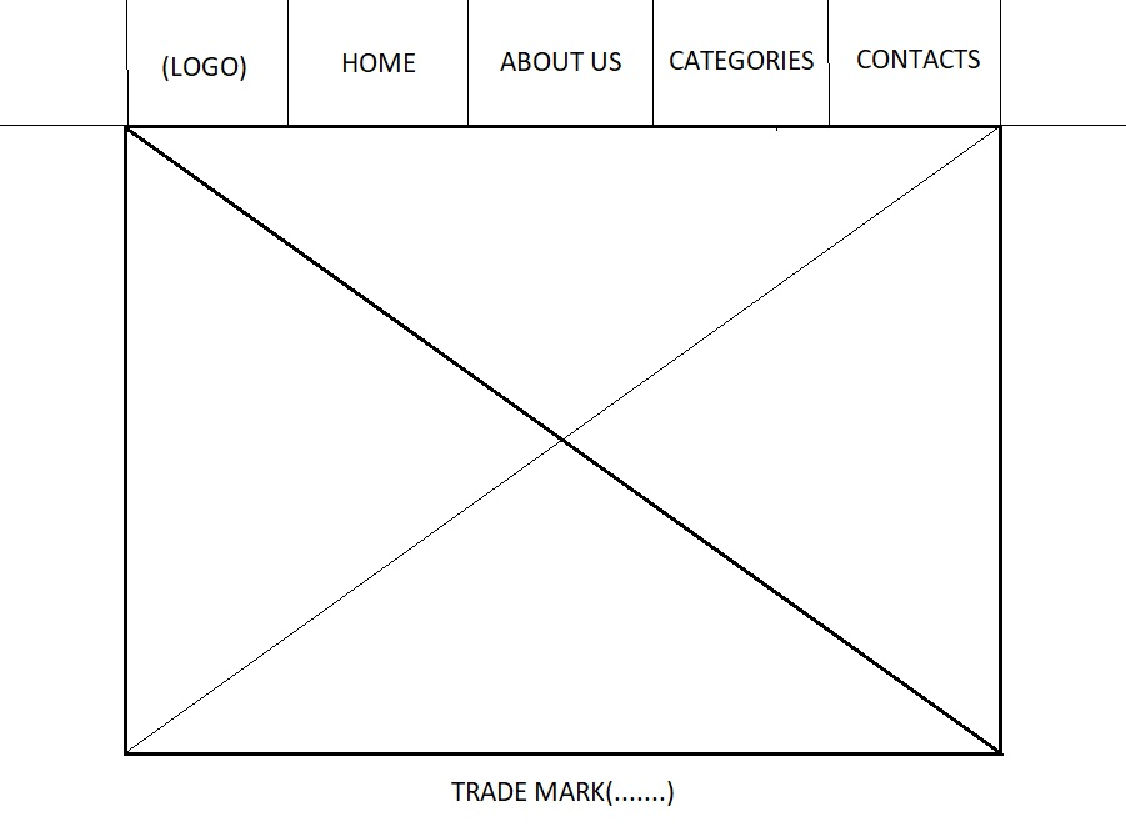
\includegraphics[width=15cm]{pic}

\newpage
\section{System specification}
\label{sec:Acting actors and objects}

% Please add the following required packages to your document preamble:
%\usepackage{graphicx}
% Please add the following required packages to your document preamble:
% \usepackage{graphicx}
\begin{table}[]
\resizebox{\textwidth}{!}{%
\begin{tabular}{|c|c|c|c|}
\hline
Actors           & Objects                                                        & Attributes                                                   & Functions                                                                                                                                                                                                                                                                                                                                                                                                                                                                        \\ \hline
Guest            & Candles                                                        & \begin{tabular}[c]{@{}c@{}}REG\\ CAR\\ ORD\end{tabular}      & \begin{tabular}[c]{@{}c@{}}REG: After entering the website, user has the option to create an account giving his/her username and password as input.\\ ORD: After entering the website, user can go to the "products" section where he can choose different products from our catalogue.\\ CAR: All of the chosen products will be placed in the shopping cart. A user can go to the shopping cart at any time and complete the purchase via bank transfer.\end{tabular}          \\ \hline
Registered users & \begin{tabular}[c]{@{}c@{}}Candles\\ User account\end{tabular} & \begin{tabular}[c]{@{}c@{}}CAR\\ ORD\\ DIS\end{tabular}      & \begin{tabular}[c]{@{}c@{}}ORD: After entering the website, user can go to the "products" section where he can choose different products from our catalogue.\\ CAR: All of the chosen products will be placed in the shopping cart. A user can go to the shopping cart at any time and complete the purchase via bank transfer.\\ DIS: Whenever a registered user buys a product, a percentage of those products price will be tranfered back into account balance.\end{tabular} \\ \hline
Admin       & \begin{tabular}[c]{@{}c@{}}Database\\ System code\end{tabular} & \begin{tabular}[c]{@{}c@{}}ACC\_MAG\\ ITEM\_MAG\end{tabular} & \begin{tabular}[c]{@{}c@{}}ACC\_MAG: Ability to alter registered users information in the database.\\ ITEM\_MAG: Ability to alter products information in the database.\end{tabular}                                                                                                                                                                                                                                                                                             \\ \hline
\end{tabular}%
}
\end{table}
 %Conclusions section
\sectionWithoutNumber{\keyWordConclusions}{conclu}
\input{conclusions.tex}

\end{document}
